% !TeX root = ../defense.tex

\section{Mathematical modelling, optimisation, case study}
\frame{\sectionpage}

\begin{frame}{Model overview}{}
    \vspace{3ex}
    \begin{center}
    \begin{tikzpicture}[node distance=1em and 8ex,font=\small]
    % flowboxes
    \node[flowbox] (urbs) {
        \fbtitle{urbs}\vphantom{yÖ}
    \nodepart{two}
        \begin{minipage}{.29\textwidth}
            \centering
            \vspace{1ex}
            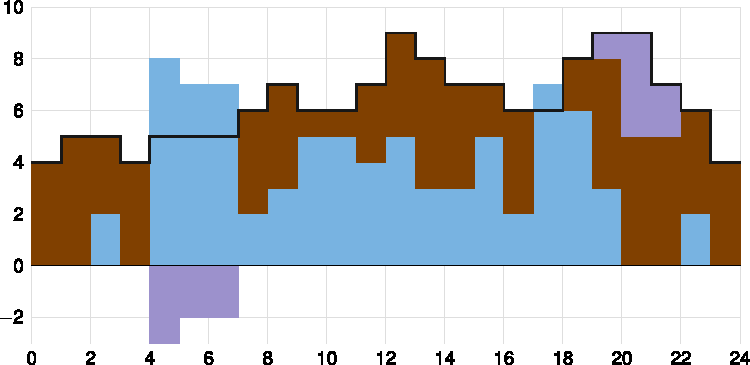
\includegraphics[width=.95\textwidth]{img/urbs/urbs-ts-graph}
            \vspace{3ex}
            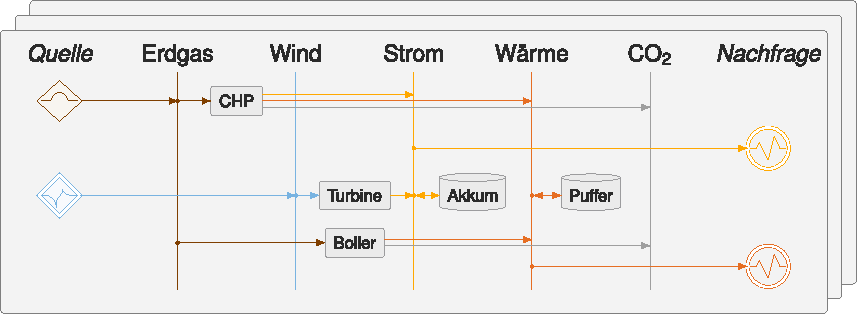
\includegraphics[width=.95\textwidth]{img/urbs/res-diagram}
            \vspace{1ex}
        \end{minipage}
    };
    \node[anchor=north west] at (urbs.south west) {\tiny \url{https://github.com/tum-ens/urbs}};

    \node[flowbox,right=of urbs] (rivus) {
        \fbtitle{rivus}\vphantom{yÖ}
    \nodepart{two}
        \begin{minipage}{.29\textwidth}
            \centering
            \vspace{-1.15ex}
            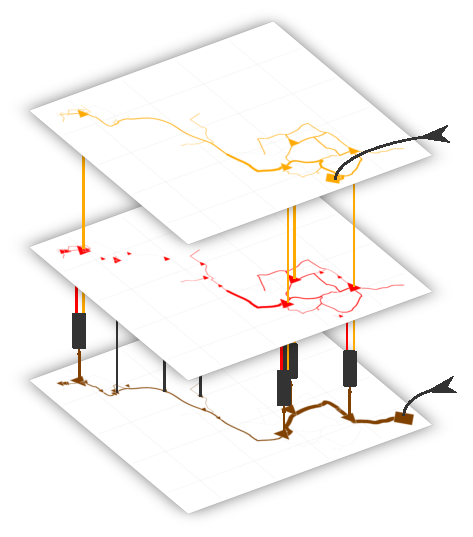
\includegraphics[width=.99\textwidth]{img/rivus/stacked-networks-half}
            \vspace{-1.15ex}
        \end{minipage}
    };
    \node[anchor=north west] at (rivus.south west) {\tiny \url{https://github.com/tum-ens/rivus}};
    \end{tikzpicture}
    \end{center}
\end{frame}

% coordinates for timeseries
\newcommand{\demandts}{( 0,4) ( 1,5) ( 2,5) ( 3,4) ( 4,5) ( 5,5) ( 6,5) ( 7,6) ( 8,7) ( 9,6) (10,6) (11,7) (12,9) (13,8) (14,7) (15,7) (16,6) (17,6) (18,8) (19,9) (20,9) (21,7) (22,6) (23,4) (24,4)}
\newcommand{\windts}{  ( 0,0) ( 1,0) ( 2,2) ( 3,0) ( 4,8) ( 5,7) ( 6,7) ( 7,2) ( 8,3) ( 9,5) (10,5) (11,4) (12,5) (13,3) (14,3) (15,5) (16,2) (17,7) (18,6) (19,3) (20,0) (21,0) (22,2) (23,0) (24,2)}

\begin{frame}{urbs}{Principle illustrated}
\begin{center}
\begin{tikzpicture}
    \begin{axis}[
        tumaxisstyle,
        x post scale=1.75,
        ymin=-3,ymax=10,
        xmin=0,xmax=24,
        xlabel={Time of day (\si{\hour})},
        ylabel={Power (\si{\MW})}]

    \path[name path=axis] (0,0) -- (24,0);

    % original wind timeseries
    \addplot[name path=ts-wind,draw=none,const plot]
        coordinates { \windts };

    \addplot[name path=ts-wind-half,draw=none,const plot,
             y filter/.code={\pgfmathparse{\pgfmathresult/2}\pgfmathresult}]
        coordinates {\windts };

    % finally: demand plot
    \addplot[name path=ts-demand,draw=demand,const plot] coordinates { \demandts };
    % slide-show

    \only<2-5>{%
        \addplot[fill=wind] fill between[of=axis and ts-wind-half];
    }
    \only<2-4>{%
        \node[jdblack!75!wind] at (12,1) {Wind turbine};
    }

    \only<3-5>{%
        \addplot[fill=gas] fill between[of=ts-wind-half and ts-demand];
    }
    \only<3-4>{%
        \node[jdwhite!95!gas] at (12,4.5) {Gas plant};
    }

    \only<4|handout:0>{%
        \draw[jdblack!75!wind,thick,darrows] (4.5, 0) -- node[right] {$\kappa_\text{w} = 4$} (4.5, 4);
        \draw[jdwhite!95!gas,thick,darrows] (20.5, 0) -- node[right] {$\kappa_\text{g} = 9$} (20.5, 9);
    }

    \only<6->{%
        \addplot[fill=wind] fill between[of=axis and ts-wind];
        \addplot [fill=gas] fill between[of=ts-wind and ts-demand,split,
                        every segment no 2/.style={fill=none},
                        every segment no 5/.style={fill=none}];
    }

    \only<7|handout:0>{%
        \draw[jdblack!75!wind,thick,darrows] (4.5, 0) -- node[right] {$\kappa_\text{w} = 8$} (4.5, 8);
        \draw[jdwhite!95!gas,thick,darrows] (20.5, 0) -- node[right] {$\kappa_\text{g} = 9$} (20.5, 9);
    }

    \only<9->{%
        \fill[storage!50] (4, 0) -- (4, -3) -- (5, -3) -- (5, -2) -- (7, -2) -- (7, 0) -- cycle; % store
        \fill[storage!50] (19,9) -- (19,8) -- (20,8) -- (20,5) -- (22, 5) -- (22, 7) -- (21, 7) -- (21, 9) -- cycle; % retreive I
    }

    \only<10->{%
        \draw[jdblack!75!wind,thick,darrows] (4.5, 0) -- node[right] {$\kappa_\text{w} = 8$} (4.5, 8);
        \draw[jdwhite!95!gas,thick,darrows] (20.5, 0) -- node[right] {$\kappa_\text{g} = 5$} (20.5, 5);
    }

    \only<11>{%
        \node[jdblack!85!storage] at (5.5, -1) {$\kappa^\text{c}_\text{s} = 7$};
        \draw[jdblack!85!storage,thick,darrows] (20.5, 5) -- node[right,near end,text=jdblack,xshift=.5em]
            {$\kappa^\text{p}_\text{s} = 4$} (20.5, 9);
    }

    \addplot[draw=demand,thick,const plot] coordinates { \demandts };
    \draw[black] (0,0) -- (24,0);
    \end{axis}
\end{tikzpicture}
\end{center}
\end{frame}

\begin{frame}{Notation as mathematical optimisation problem}
    \begin{align*}
        \text{Sets\quad}
            & t\in T,\ p\in P,\ s\in S,\ \dots
            \\
    \uncover<+->{
        \text{Parameters\quad}
            & d_t
              \uncover<+->{,\ k^\text{fix}_p,\ k^\text{fix,c}_s,\ k^\text{fix,p}_s}
              \uncover<+->{,\ k^\text{var}_p,\ k^\text{var}_s,\ \ldots}
            \\
    }
    \uncover<+->{
        \text{Variables\quad}
            & \kappa_p,\ \kappa_s^\text{c},\ \kappa_s^\text{p}
              \uncover<+->{,\ \epsilon_{pt},\ \epsilon_{st}^\text{in},\ \epsilon_{st}^\text{out},\ \epsilon_{st}^\text{con},\ \ldots}
            \\
    }
    \uncover<+->{
        \text{Objective\quad}
            & \min \sum_{p \in P} \Big( k^\text{fix}_p \kappa_p + \sum_{t\in T} k^\text{var} \epsilon_{pt} \Big) + \\
            & \phantom{\min} \sum_{s \in S} \Big( k^\text{fix,c}_s \kappa_s^\text{c} + k^\text{fix,p}_s \kappa_s^\text{p} + \sum_{t\in T} k_s^\text{var} \big(\epsilon^\text{in}_{st} + \epsilon^\text{out}_{st} \big) \Big)
            \\
    }
    \uncover<+->{
        \text{Constraints\quad}
            & \st\; \forall t\in T\colon\ \sum_{p\in P} \epsilon_{pt} + \sum_{s\in S} \big( \epsilon^\text{out}_{st} - \epsilon^\text{in}_{st} \big) = d_t \\
            & \phantom{\st\;} \ldots
    }
    \end{align*}
\end{frame}

\begin{frame}{Standard form of linear optimisation problems (LP)}
    \begin{alertblock}{Generic form}
        \vspace*{-1.5em}
        \begin{align*}
            \min_{\bs x}\ & z = \bs c\T \bs x \\
            \st\; & \bs A \bs x \leq \bs b
        \end{align*}

        \centering
        with $\bs x \in \R^n$, $\bs A \in \R^{m \times n}$,\\\, $\bs b \in \R^m$, $\bs c \in \R^n$.
        \vspace*{1ex}
    \end{alertblock}
\end{frame}

\begin{frame}{Mixed-integer linear programming (MILP)}
    \vspace*{-3em}
    \begin{columns}[onlytextwidth,t]
    \column{.5\textwidth-.25cm}
        \begin{center}
        \begin{tikzpicture}[scale=.85]
        \begin{axis}[
                tumaxisstyle,
                xlabel={$x_i$}, ylabel={$z$ (absolute)},
                xmin=-40, xmax=1000, ymin=0, ymax=600,
                y post scale=0.65, ylabel near ticks, clip=false,
                grid=both, xticklabels={,0,$m$,,,,$M$}, yticklabels={,0}]

            \addplot[color=tumblue,thick] coordinates { (0,0) (1000, 200) };
            \node at (axis cs:1000,200) [anchor=west,text=tumblue] {LP};
            \only<4->{
                \addplot[color=jdgreen,thick,dotted] coordinates { (0, 0) (0, 300) (200, 340) };
                \addplot[color=jdgreen,thick] coordinates { (200, 340) (1000, 500) };
                \draw[densely dotted]
                    (axis cs:300,360)
                 -| (axis cs:500,400)
                    node[near end,below right]
                    {$k_i^\text{var}$};

                \draw[densely dotted]
                    (axis cs:-15,300)
                 -- (axis cs:30,300)
                    node[near end,below right]
                    {$k_i^\text{fix}$};
            }
            \node at (axis cs:1000,500) [text=jdgreen,anchor=west] {{\visible<4->{MILP}}};
            \draw (axis cs:-40,0) -- (axis cs:1000,0);
        \end{axis}
        \end{tikzpicture}
        \end{center}
        \vspace*{-2.5em}

        \begin{align*}
        \color{tumblue}\text{LP\quad} z &\color{tumblue}= k_i^\text{var} x_i \\
         \color{tumblue}x_i &\color{tumblue}\leq M \\[3pt]
        \uncover<4->{
        \color{jdgreen}\text{MILP\quad} z &\color{jdgreen}= k_i^\text{fix} y_i + k_i^\text{var} x_i \\
        \color{jdgreen}y_i &\color{jdgreen}\in \{0,1\} \\
        \color{jdgreen}m\, y_i &\color{jdgreen}\leq x_i \leq M\, y_i
        }
        \end{align*}

    \column{.5\textwidth-.25cm}
        \begin{center}
        \begin{tikzpicture}[scale=.85]
        \begin{axis}[
                tumaxisstyle,
                xlabel={$x_i$}, ylabel={$z/x_i$ (specific)},
                xmin=-40, xmax=1000, ymin=0, ymax=600,
                y post scale=0.65, ylabel near ticks, clip=false,
                grid=both, xticklabels={,0,$m$,,,,$M$}, yticklabels={,0,$k^\text{var}_i$}]

            \node at (axis cs:1000,200) [anchor=west,text=tumblue,yshift=-.25ex] {{\visible<2->{LP}}};
            \only<2->{
                \addplot[color=tumblue,thick] coordinates { (0,200) (1000, 200) };
            }
            \only<3->{
                \addplot[color=jdgreen,thick,dotted,domain=100:200] {200 + 40000/x};
                \addplot[color=jdgreen,thick,domain=200:1000] {200 + 40000/x};
            }
            \node at (axis cs:1000,240) [text=jdgreen,anchor=west,yshift=.25ex] {{\visible<3->{MILP}}};
            \draw (axis cs:-40,0) -- (axis cs:1000,0);
        \end{axis}
        \end{tikzpicture}
        \end{center}
        \vspace*{-2.5em}

        \begin{align*}
        \uncover<2->{
        \color{tumblue}\text{LP\quad} \frac{z}{x_i} &\color{tumblue} = k_i^\text{var} \equiv \text{const} \\[3pt]}
        \uncover<3->{
        \color{jdgreen}\text{MILP\quad} \frac{z}{x_i} &\color{jdgreen} = k_i^\text{var} + \frac{k_i^\text{fix}}{x_i}}
        \end{align*}

    \end{columns}
\end{frame}

\begin{frame}{rivus}{Principle illustrated}
    \begin{columns}[onlytextwidth,t]
    \column{.5\textwidth-.25cm}
        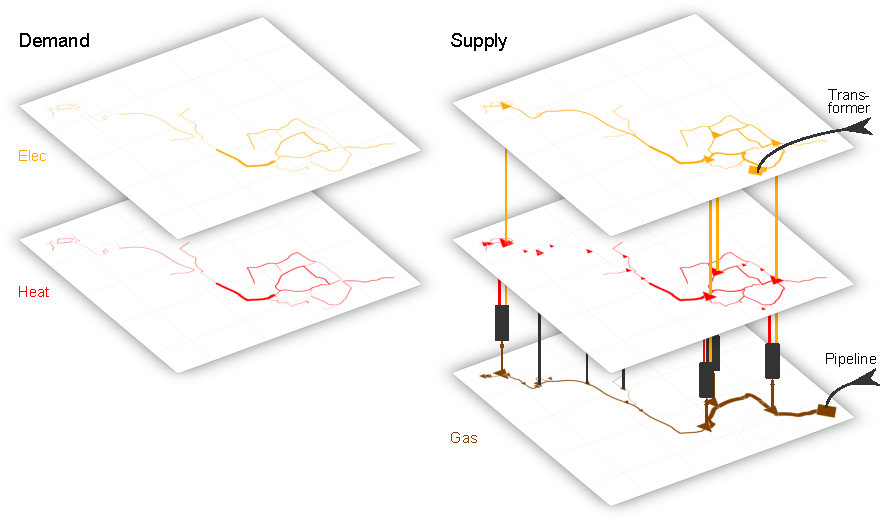
\includegraphics[width=\columnwidth,clip=true,trim={0 0 215 0}]{img/rivus/stacked-networks}
    \column{.5\textwidth-.25cm}
    \uncover<2->{%
        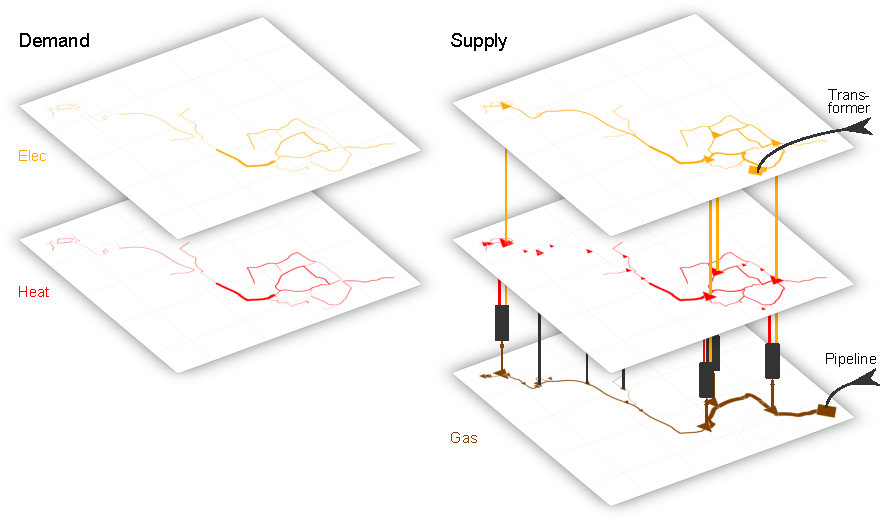
\includegraphics[width=\columnwidth,clip=true,trim={210 0 0 0}]{img/rivus/stacked-networks}
    }
    \end{columns}
\end{frame}

\fullframegraphics[\color{jdlightestgrey}\hypersetup{urlcolor=jdlighterblue}
Haag i. OB,
data
    \href{http://www.openstreetmap.org/copyright}{OpenStreetMap contributors}
   (\href{http://opendatacommons.org/licenses/odbl/}{ODbL}),
style
    \href{https://github.com/charleyglynn/OSM-Shapefile-QGIS-stylesheets}{Charley Glynn}
   (\href{http://creativecommons.org/licenses/by-sa/3.0/}{CC BY-SA})]
{img/haag/haag-i-ob}{%
    \uncover<2>{%
    \node[at=(current page.north west),
          xshift=3.5cm,yshift=-0.9cm,
          font=\footnotesize,text=jddarkergrey,fill=yellow,
          fill opacity=.75,text opacity=1,
          inner xsep=3pt, inner ysep=5pt,
          rounded corners=2pt] {Moosham};
    }%
}

\begin{frame}{Input data \textbf{rivus}}
    \begin{columns}
        \column{\squeezethree}
        	\centering
        	\textcolor{elec}{Electricity} \vphantom{gÖ}
        	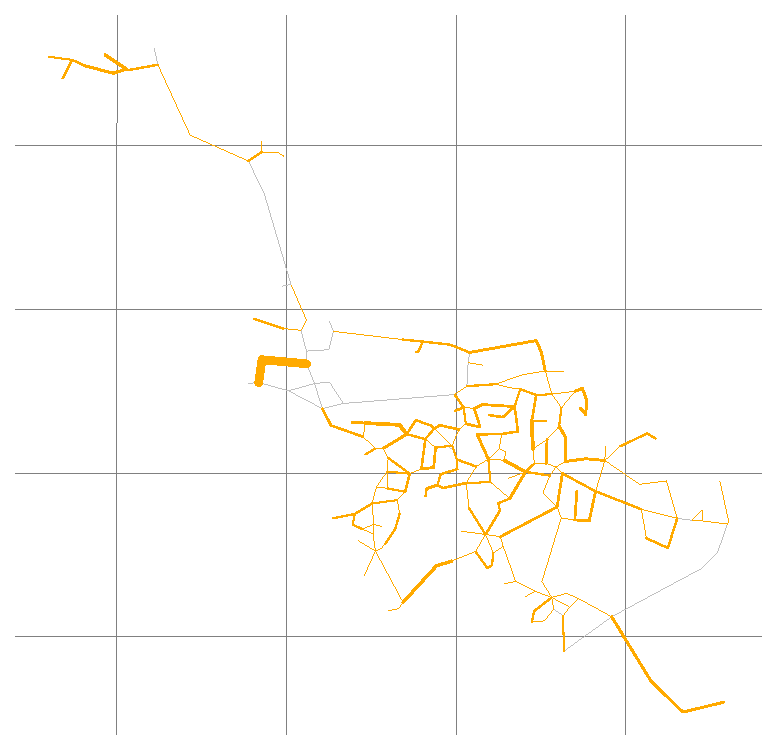
\includegraphics[width=\squeezethree]{img/haag/scenario_no_electric_heating-peak-Elec}
        \column{\squeezethree}
        	\centering
        	\textcolor{heat}{Heat} \vphantom{gÖ}
        	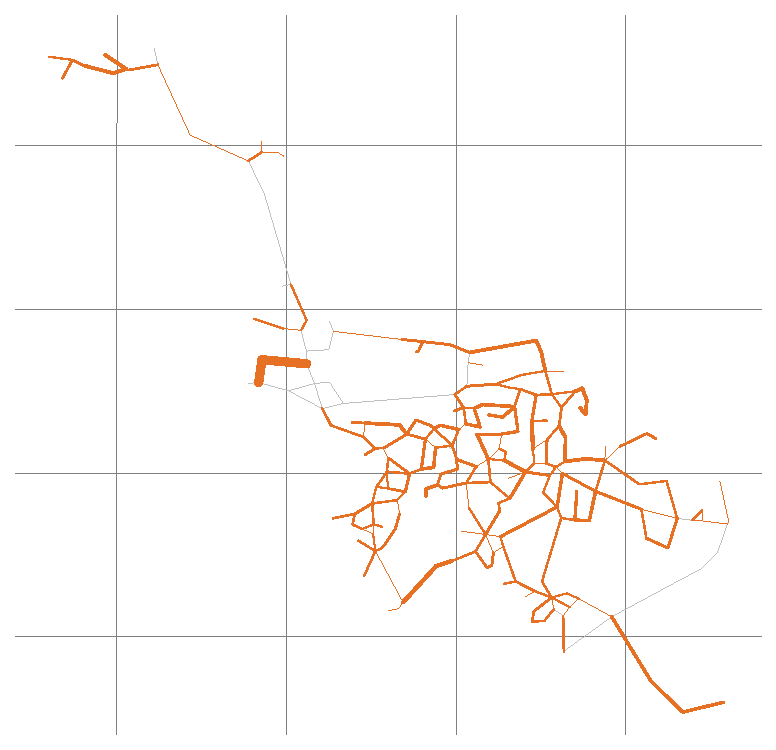
\includegraphics[width=\squeezethree]{img/haag/scenario_no_electric_heating-peak-Heat}
        \column{\squeezethree}
    \end{columns}

    \begin{center}
        \raggedright\qquad
        Light industry (Schletter) biggest single consumer
    \end{center}

    {\tiny \url{https://github.com/tum-ens/rivus}/\texttt{data/haag15}}
\end{frame}

\begin{frame}{Result \textbf{rivus} -- Capacities in scenario \scenario{base}}
    \begin{columns}
        \column{\squeezethree}
        	\centering
        	\textcolor{elec}{Electricity} \vphantom{gÖ}
        	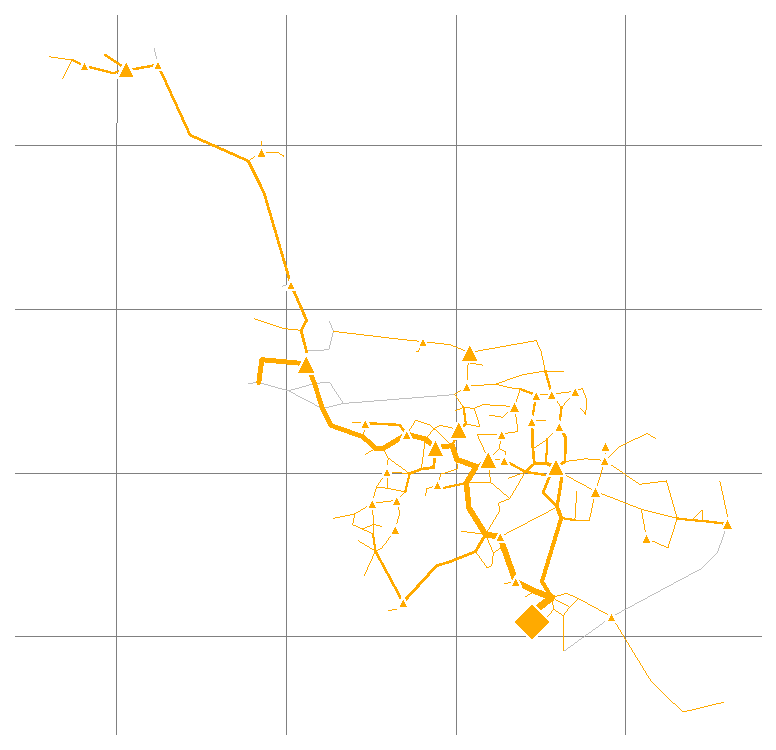
\includegraphics[width=\squeezethree]{img/haag/scenario_no_electric_heating-caps-Elec}
        \column{\squeezethree}
        	\centering
        	\textcolor{heat}{Heat} \vphantom{gÖ}
        	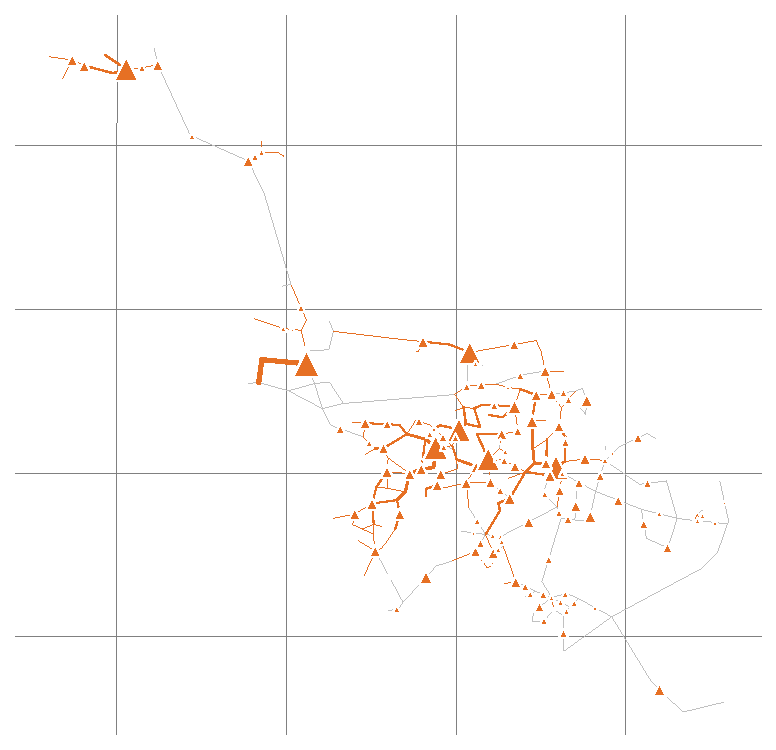
\includegraphics[width=\squeezethree]{img/haag/scenario_no_electric_heating-caps-Heat}
        \column{\squeezethree}
        	\centering
        	\textcolor{gas}{Gas} \vphantom{gÖ}
        	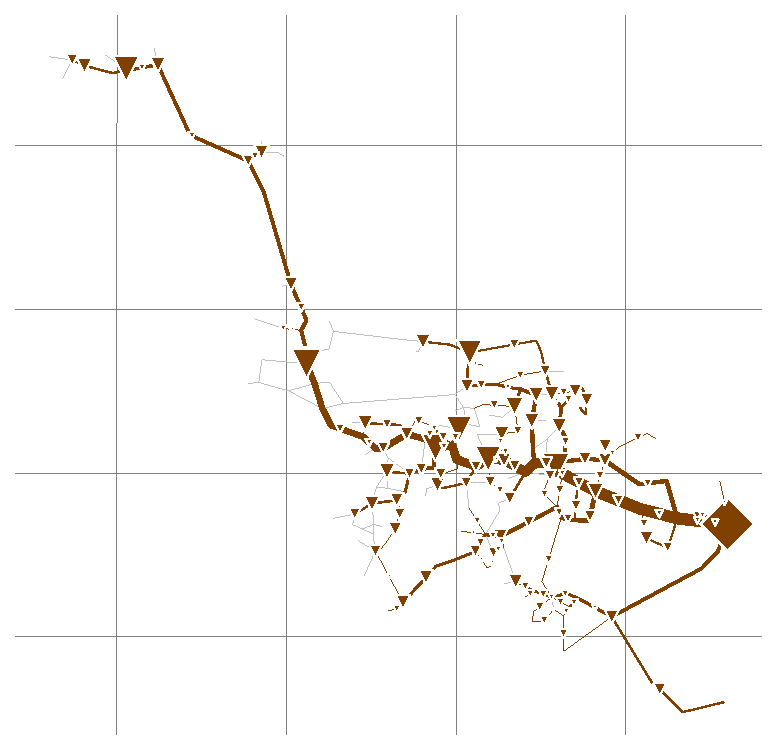
\includegraphics[width=\squeezethree]{img/haag/scenario_no_electric_heating-caps-Gas}
    \end{columns}

    \begin{center}
        Full networks for electricity and gas, several local heating networks
    \end{center}

    {\tiny \url{https://github.com/tum-ens/rivus}/\texttt{runhg15.py:scenario\_no\_electric\_heating()}}
\end{frame}

\begin{frame}{Result \textbf{rivus} -- Capacities in scenario \scenario{future}}
    \begin{columns}
        \column{\squeezethree}
        	\centering
        	\textcolor{elec}{Electricity} \vphantom{gÖ}
        	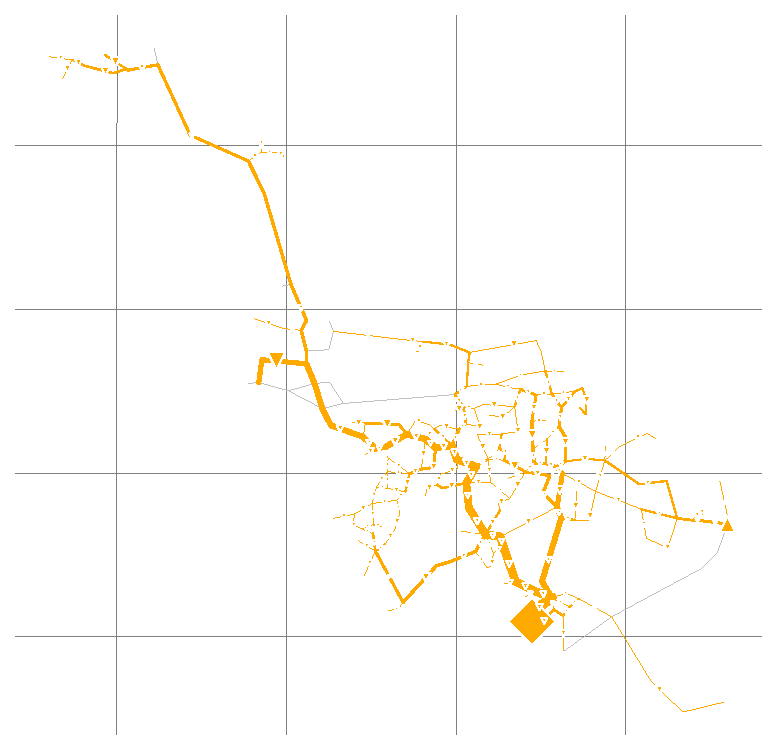
\includegraphics[width=\squeezethree]{img/haag/scenario_renovation-caps-Elec}
        \column{\squeezethree}
        	\centering
        	\textcolor{heat}{Heat} \vphantom{gÖ}
        	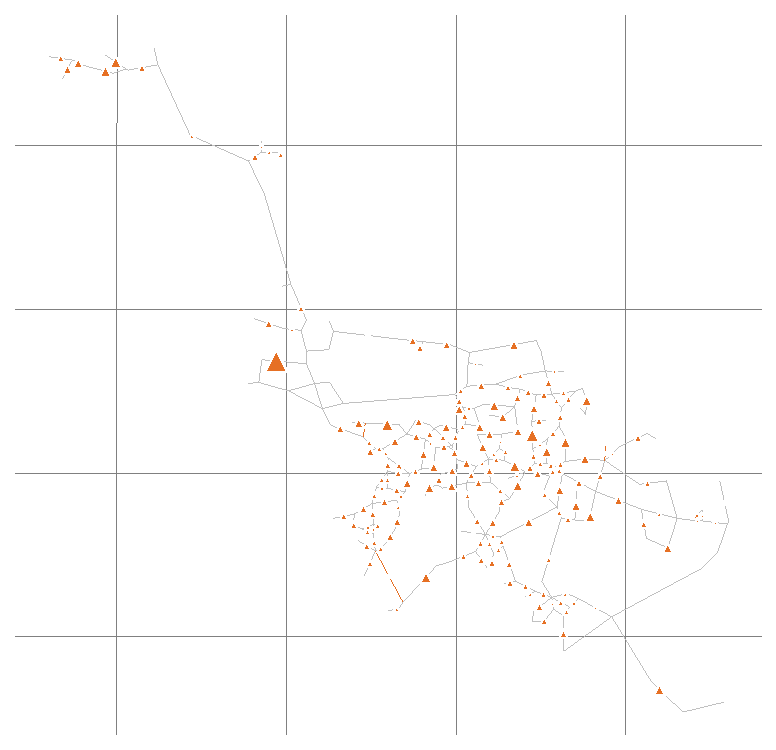
\includegraphics[width=\squeezethree]{img/haag/scenario_renovation-caps-Heat}
        \column{\squeezethree}
        	\centering
        	\textcolor{gas}{Gas} \vphantom{gÖ}
        	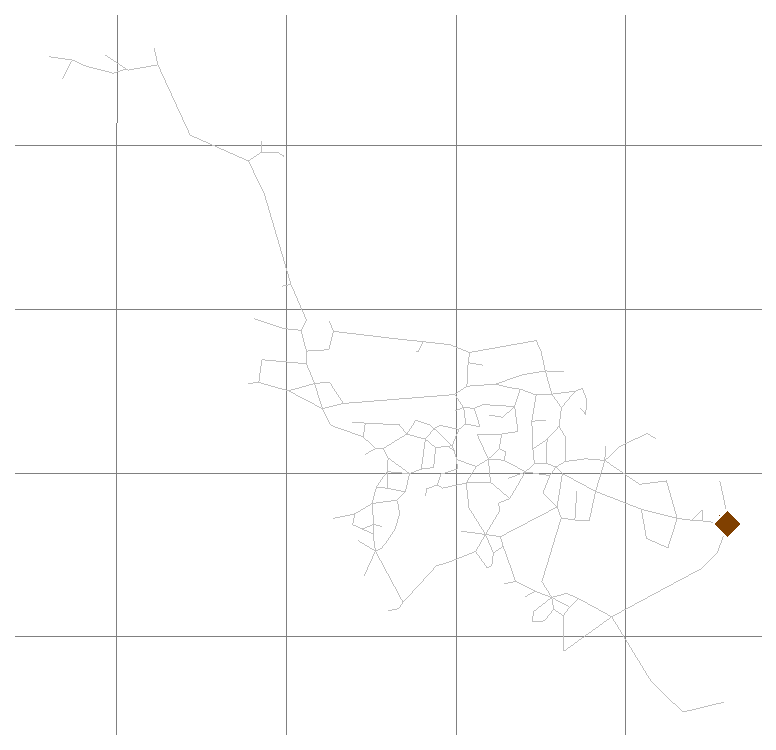
\includegraphics[width=\squeezethree]{img/haag/scenario_renovation-caps-Gas}
    \end{columns}

    \begin{center}
        Strong electricity grid, no gas network, only heat pumps
    \end{center}

    {\tiny \url{https://github.com/tum-ens/rivus}/\texttt{runhg15.py:scenario\_renovation()}}
\end{frame}

\begin{frame}{Result \textbf{urbs} -- 1 week electricity in scenarios \scenario{base}}
    \begin{center}
        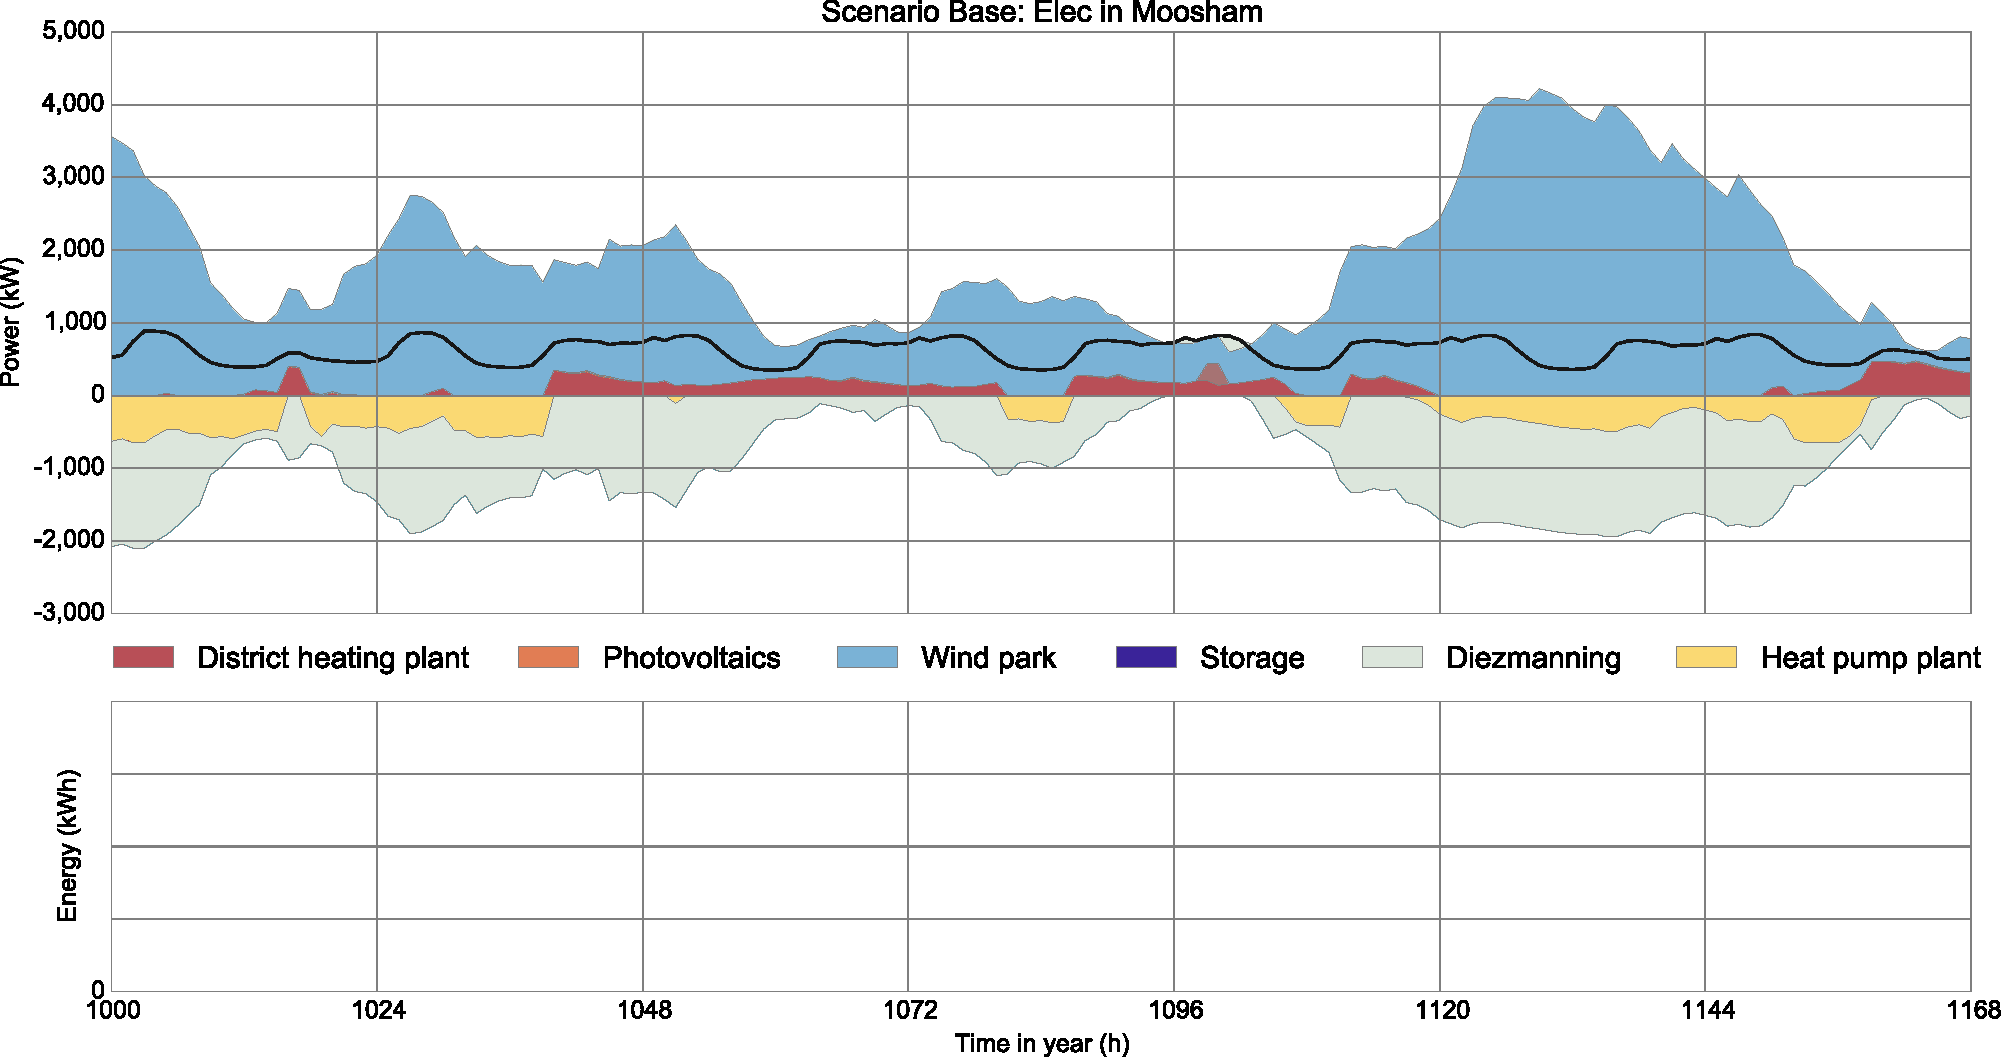
\includegraphics[width=.95\textwidth]{img/haag/scenario_base-Elec-Moosham-spr_edit}
    \end{center}
    \vspace{-1em}
    {\tiny \url{https://github.com/ojdo/urbs/tree/haag15}/\texttt{rivhg15.py:scenario\_base()}}
\end{frame}

\begin{frame}{Result \textbf{urbs} -- 1 week electricity in scenario \scenario{cheap battery}}
    \begin{center}
        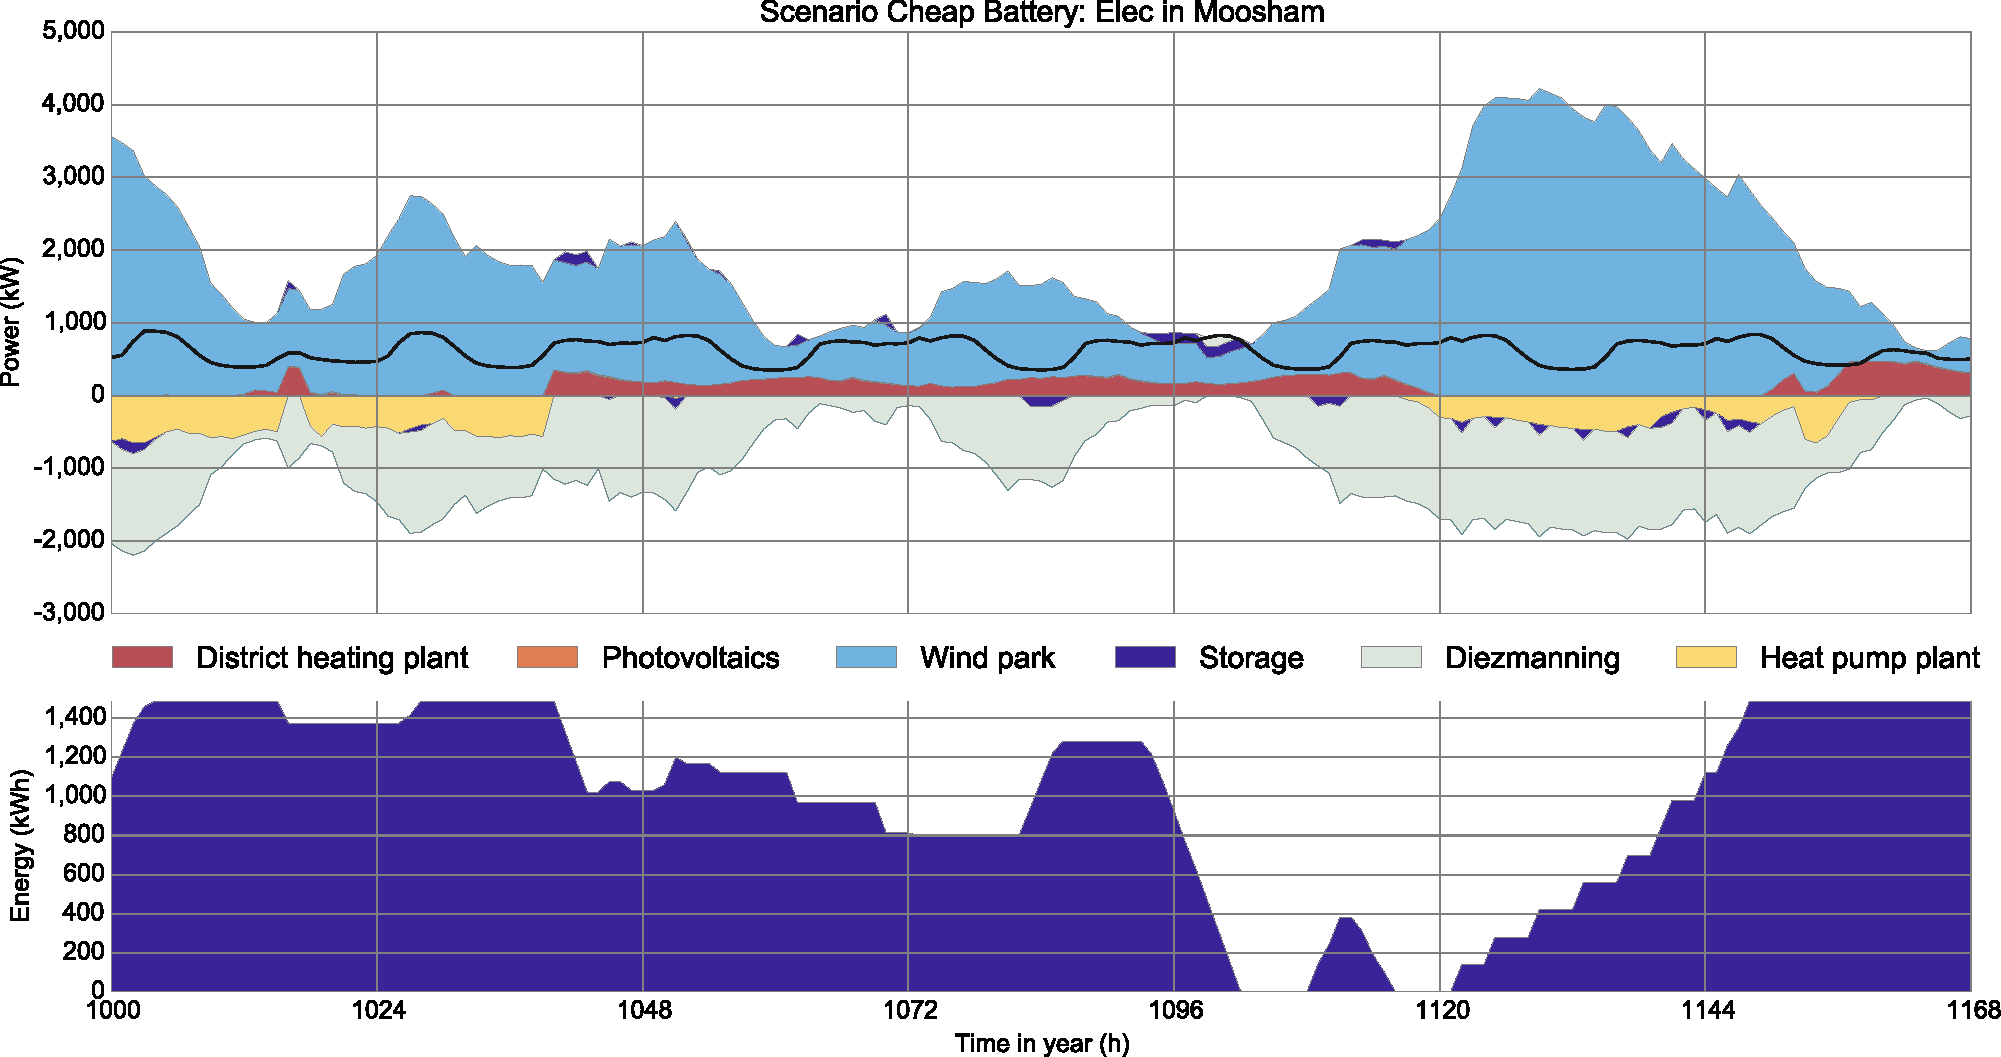
\includegraphics[width=.95\textwidth]{img/haag/scenario_cheap_battery-Elec-Moosham-spr_edit}
    \end{center}
    \vspace{-1em}
    {\tiny \url{https://github.com/ojdo/urbs/tree/haag15}/\texttt{rivhg15.py:scenario\_cheap\_battery()}}
\end{frame}
